\documentclass[11pt,letterpaper]{article}
\usepackage[top=3cm, bottom=2cm, left=2cm, right=2cm, columnsep=20pt]{geometry}
\usepackage{pdfpages}
\usepackage{graphicx}
\usepackage{etoolbox}
\apptocmd{\sloppy}{\hbadness 10000\relax}{}{}
% \usepackage[numbers]{natbib}
\usepackage[T1]{fontenc}
\usepackage{ragged2e}
\usepackage[french]{babel}
\usepackage{listings}
\usepackage{color}
\usepackage{soul}
\usepackage[utf8]{inputenc}
\usepackage[export]{adjustbox}
\usepackage{caption}
\usepackage{amsmath}
\usepackage{amssymb}
\usepackage{float}
\usepackage{csquotes}
\usepackage{fancyhdr}
\usepackage{wallpaper}
\usepackage{siunitx}
\usepackage[indent]{parskip}
\usepackage{textcomp}
\usepackage{gensymb}
\usepackage{multirow}
\usepackage[hidelinks]{hyperref}
\usepackage{abstract}


\renewcommand{\abstractnamefont}{\normalfont\bfseries}
\renewcommand{\abstracttextfont}{\normalfont\itshape}
\usepackage{titlesec}
\titleformat{\section}{\large\bfseries}{\thesection}{1em}{}
\titleformat{\subsection}{\normalsize\bfseries}{\thesubsection}{1em}{}
\titleformat{\subsubsection}{\normalsize\bfseries}{\thesubsubsection}{1em}{}

\usepackage{xcolor}
\definecolor{codegreen}{rgb}{0,0.6,0}
\definecolor{codegray}{rgb}{0.5,0.5,0.5}
\definecolor{codepurple}{rgb}{0.58,0,0.82}
\definecolor{backcolour}{rgb}{0.95,0.95,0.92}
\lstdefinestyle{mystyle}{
    backgroundcolor=\color{backcolour},   
    commentstyle=\color{codegreen},
    keywordstyle=\color{magenta},
    numberstyle=\tiny\color{codegray},
    stringstyle=\color{codepurple},
    basicstyle=\ttfamily\footnotesize,
    breakatwhitespace=false,         
    breaklines=true,                 
    captionpos=b,                    
    keepspaces=true,                 
    numbers=left,                    
    numbersep=5pt,                  
    showspaces=false,                
    showstringspaces=false,
    showtabs=false,                  
    tabsize=2
}
\lstset{style=mystyle}

\usepackage[most]{tcolorbox}
\newtcolorbox{note}[1][]{
  enhanced jigsaw,
  borderline west={2pt}{0pt}{black},
  sharp corners,
  boxrule=0pt, 
  fonttitle={\large\bfseries},
  coltitle={black},
  title={Note:\ },
  attach title to upper,
  #1
}

%----------------------------------------------------

\setlength{\parindent}{0pt}
\DeclareCaptionLabelFormat{mycaptionlabel}{#1 #2}
\captionsetup[figure]{labelsep=colon}
\captionsetup{labelformat=mycaptionlabel}
\captionsetup[figure]{name={Figure }}
\newcommand{\inlinecode}{\normalfont\texttt}
\usepackage{enumitem}
\setlist[itemize]{label=\textbullet}

\begin{document}
\begin{titlepage}
\center

\begin{figure}
    \ThisULCornerWallPaper{.4}{Polytechnique_signature-RGB-gauche_FR.png}
\end{figure}
\vspace*{2 cm}

\textsc{\Large \textbf{PHS3910 --} Techniques expérimentales et instrumentation}\\[0.5cm]
\large{\textbf{Équipe : Lundi 03}}\\[1.5cm]

\rule{\linewidth}{0.5mm} \\[0.5cm]
\Large{\textbf{Spectromètre}} \\[0.2cm]
\text{Fiche technique}\\
\rule{\linewidth}{0.2mm} \\[2.3cm]

\large{\textbf{Présenté à}\\
  Jean Provost\\
  Lucien Weiss\\[2.5cm]
  \textbf{Par :}\\
  Émile \textbf{Guertin-Picard} (2208363)\\
  Philippine \textbf{Beaubois} (2211153)\\
  Marie-Lou \textbf{Dessureault} (2211129)\\
  Maxime \textbf{Rouillon} (2213291)\\[3cm]}

\large{\today\\
Département de Génie Physique\\
Polytechnique Montréal\\}

\end{titlepage}

%----------------------------------------------------

\tableofcontents
\pagenumbering{roman}
\newpage

\pagestyle{fancy}
\setlength{\headheight}{14pt}
\renewcommand{\headrulewidth}{0pt}
\fancyfoot[R]{\thepage}

\pagestyle{fancy}
\fancyhf{}
\renewcommand{\headrulewidth}{1pt}
\fancyhead[L]{\textbf{PHS3910}}
\fancyhead[C]{Fiche technique du microscope}
\fancyhead[R]{\today}
\fancyfoot[R]{\thepage}

\pagenumbering{arabic}
\setcounter{page}{1}

%----------------------------------------------------

\section{Description générale et spécifications}

Cette fiche technique, à la demande du Gouvernement du Québec, présente les caractéristiques 
d'un microscope servant au suivi de microparticules contaminants l'environnement près de 
l'usine Polyfab \textcolor{red}{lol}. Les composantes principales sont un laser 405 nm (CPS405)
pour illuminer les fluorophores dans les échantillons, un objectif de microscope (grossissement 
$M = 20$, aperture NA $= 0.4$) pour le grossissement, puis une lentille tube de 150 mm de focale
(LA1433-A-ML) pour converger les rayons sortants de l'objectif sur le capteur d'une caméra CMOS 
(CS165MU) pour l'analyse \textcolor{red}{Source Thorlabs}. Ce système présente une résolution
théorique de 1.012 µm. Afin d'analyser des particules d'environ cette taille, un traitement
numérique est fait pour extraire la taille des particules du mouvement brownien filmé, avec 
une résolution sous-pixellaire. Avec ce procédé, le microscope peut détecter des tailles de 
particules dans la plage  \textcolor{red}{XX - XX} µm. Suite à la caractérisation de particules 
de 1 µm, l'erreur sur la valeur identifiée est de \textcolor{red}{XX $\pm$ XX} µm.
Pour la caractérisation de particules de 10 µm, l'erreur sur la valeur identifiée est de 
\textcolor{red}{XX $\pm$ XX} µm. Le système, monté sur table optique et utilisable dans le noir 
seulement, a des dimensions de \textcolor{red}{$600 \times 90 \times 200$} mm. Sans compter la
table, il a pour coût total 1483.59 \$, prix qui peut être réduit par l'usage d'impression 3D.

% Source Thorlabs : https://www.thorlabs.com

\begin{figure}[H]
  \centering
  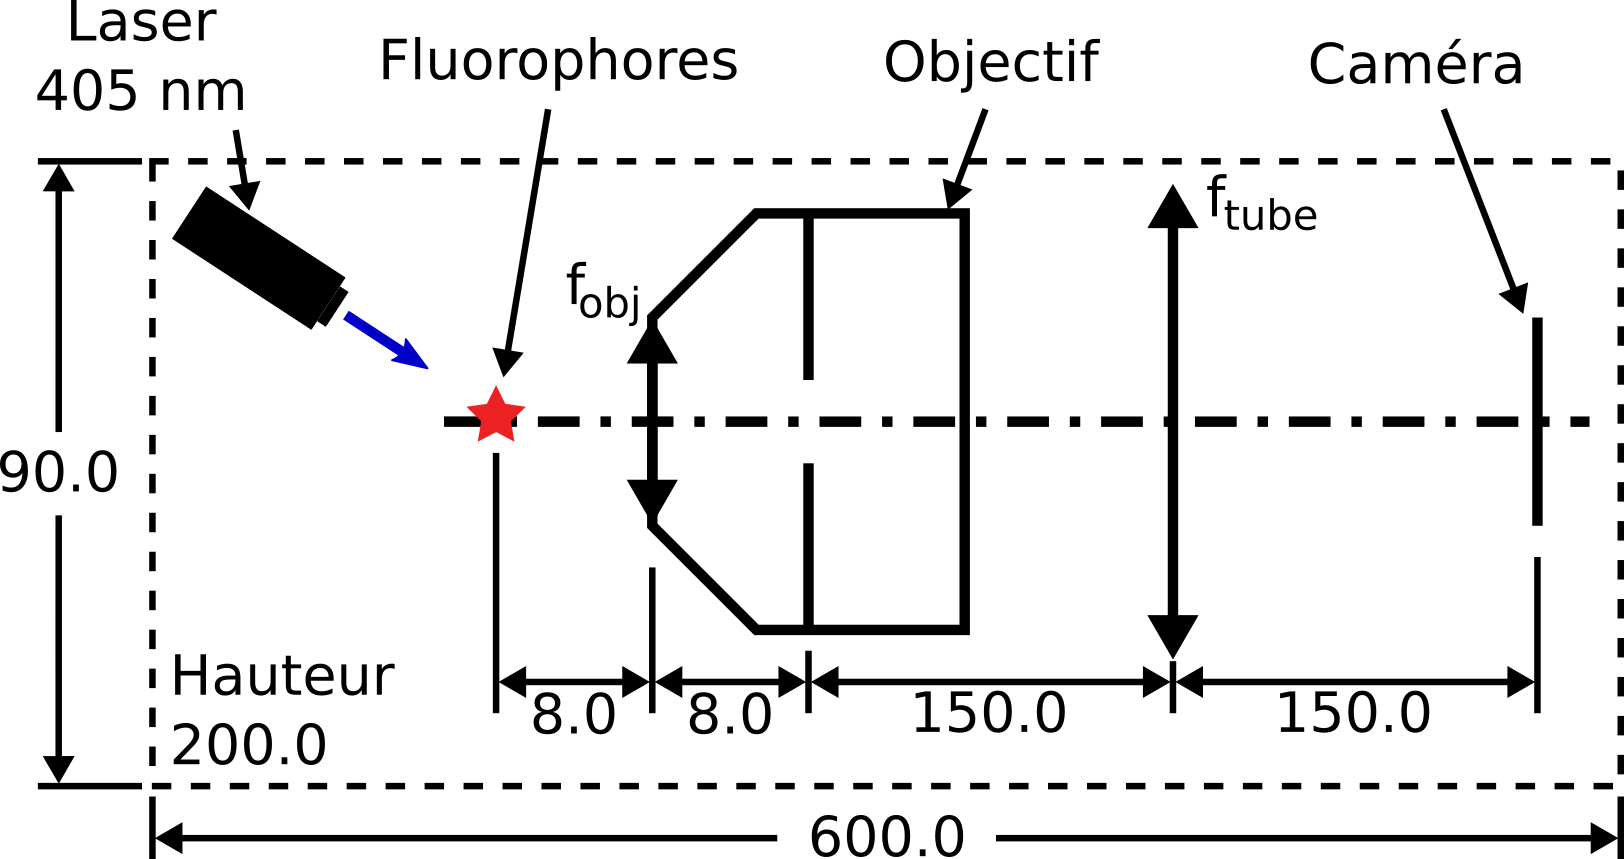
\includegraphics[scale=2.8]{schema_fiche_tech.png}
  \caption{Schéma du microscope avec les dimensions critiques. Toutes les dimensions sont en millimètres avec une tolérance de $\pm$ 1 mm.}
  \label{}
\end{figure}



\section{Rapports de tests}

\subsection{Résolution sans analyse numérique}

\textcolor{red}{ce qui était dans le rapport préliminaire}


\subsection{Caractérisation de la taille de particules}

\textcolor{red}{Acquisition de données (paramètres d'acquisition, traitement des lost frames)}

\textcolor{red}{}

\subsubsection{Paramètres utilisés}



\subsection{Étude des coûts}

\begin{table}[!ht]
    \centering
    \caption{Liste des pièces et coûts totaux pour le microscope sur table optique
    \textcolor{red}{Source Thorlabs}.}
    \begin{tabular}{|l|l|l|l|l|}
    \hline
        ID pièce & Description & Qté & \$ CAD & Total ind. \\ \hline\hline
        KM100S & Montage à réseau de diffraction & 1 & \$130.45 & \$130.45 \\ \hline
        CS165MU & Caméra CMOS monochrome & 1 & \$667.01 & \$667.01 \\ \hline
        - & Objectif de microscope & 1 & \$10.00 & \$10.00 \\ \hline
        420FDL12 & Filtre passe-long & 1 & \$36.29 & \$36.29 \\ \hline
        LA1433-A-ML & Lentille tube f = 150.0 mm & 1 & \$71.42 & \$71.42 \\ \hline
        CPS405 & Laser bleu 405 nm & 1 & \$312.07 & \$312.07 \\ \hline
        LMR1 & Trou taraudé pour lentilles & 2 & \$22.89 & \$45.79 \\ \hline
        TR3-P5 & 5 tiges 3 po pour optiques & 1 & \$38.50 & \$38.50 \\ \hline
        PH4 & Base pour tiges d'optique 4 po & 4 & \$14.83 & \$59.33 \\ \hline
        PH3 & Base pour tiges d'optique 3 po & 1 & \$13.37 & \$13.37 \\ \hline
        BA1 & Pied de montage optique & 1 & \$8.42 & \$8.42 \\ \hline
        BA1S & Pied de montage optique & 2 & \$7.83 & \$15.65 \\ \hline
        BA2 & Pied de montage optique & 1 & \$11.26 & \$11.26 \\ \hline
        VC1 & Pince en V & 1 & \$64.04 & \$64.04 \\ \hline\hline
        ~ & ~ & ~ & Total : & \$1,483.59 \\ \hline
    \end{tabular}
\end{table}

% Source Thorlabs : https://www.thorlabs.com

% \bibliographystyle{unsrtnat}
% \bibliography{My_Library}

\end{document}
